\section{Verification of MEPS ensemble members}\label{sec:variation}
%%%%%%%%% image SWC retrieved %%%%%%%%%%%%%%
% !TeX spellcheck = en_GB

%%%%%%%
\begin{figure}[t]
	\centering
    % 20/12
		\begin{subfigure}[t]{\textwidth}		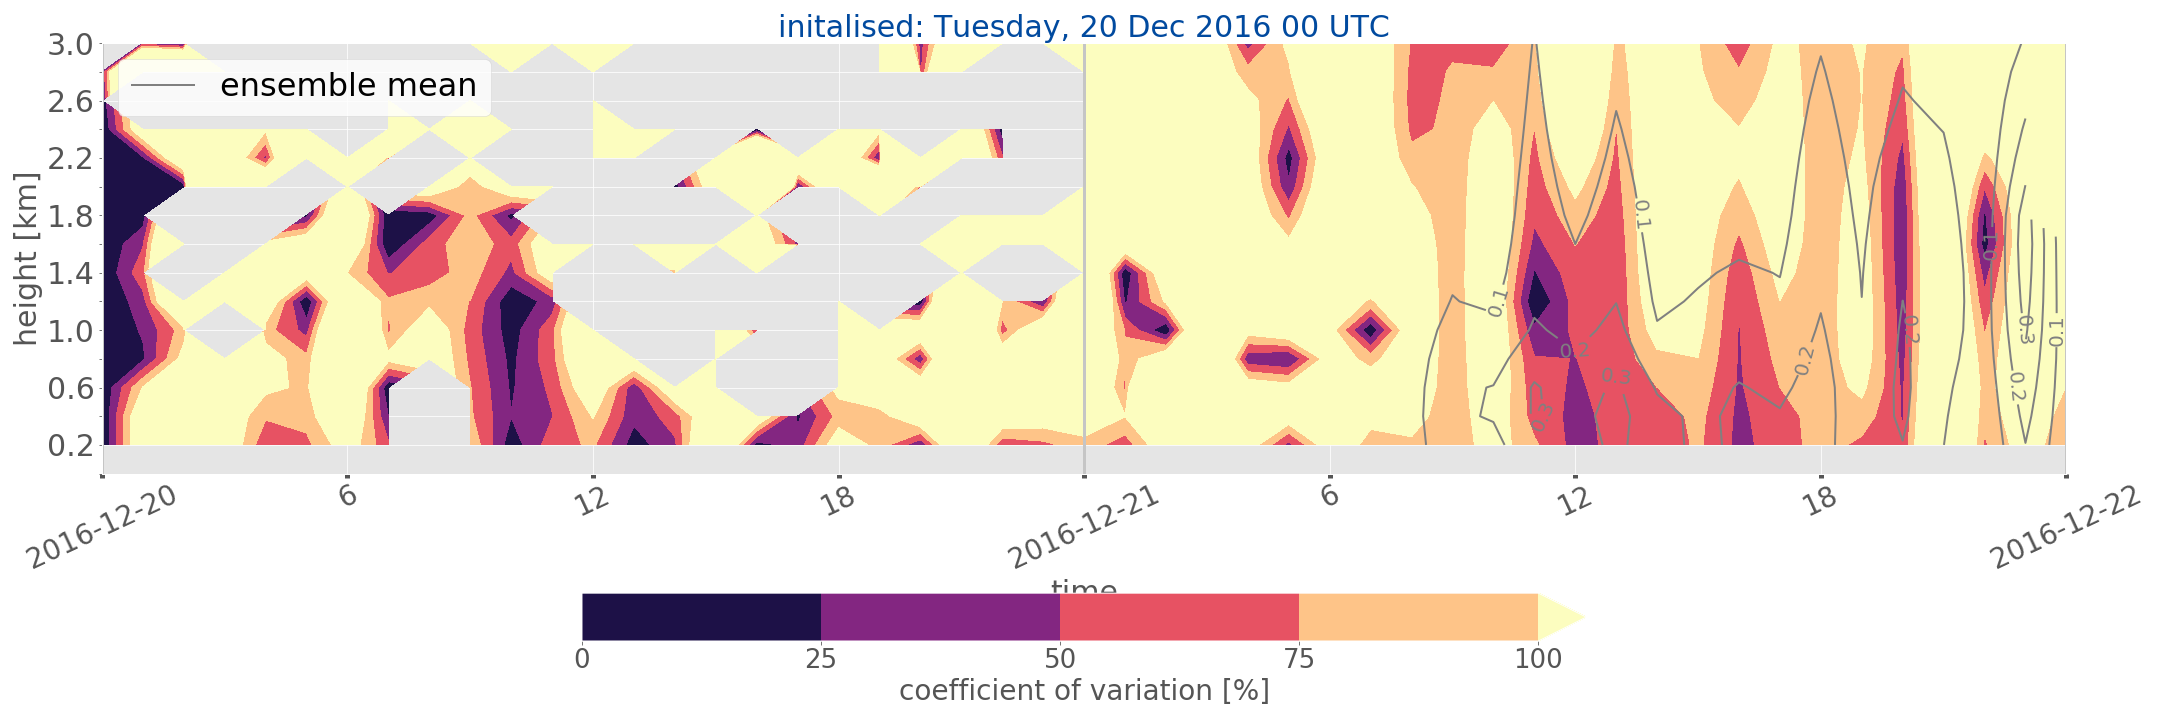
\includegraphics[trim={0.cm 5.3cm 0cm 0cm},clip,width=\textwidth]{./fig_variation/20161220}
			\caption{}\label{fig:ens_vari20}
		\end{subfigure}
%\end{figure}
%\begin{figure}\ContinuedFloat
    % 21/12
		\begin{subfigure}[t]{\textwidth}		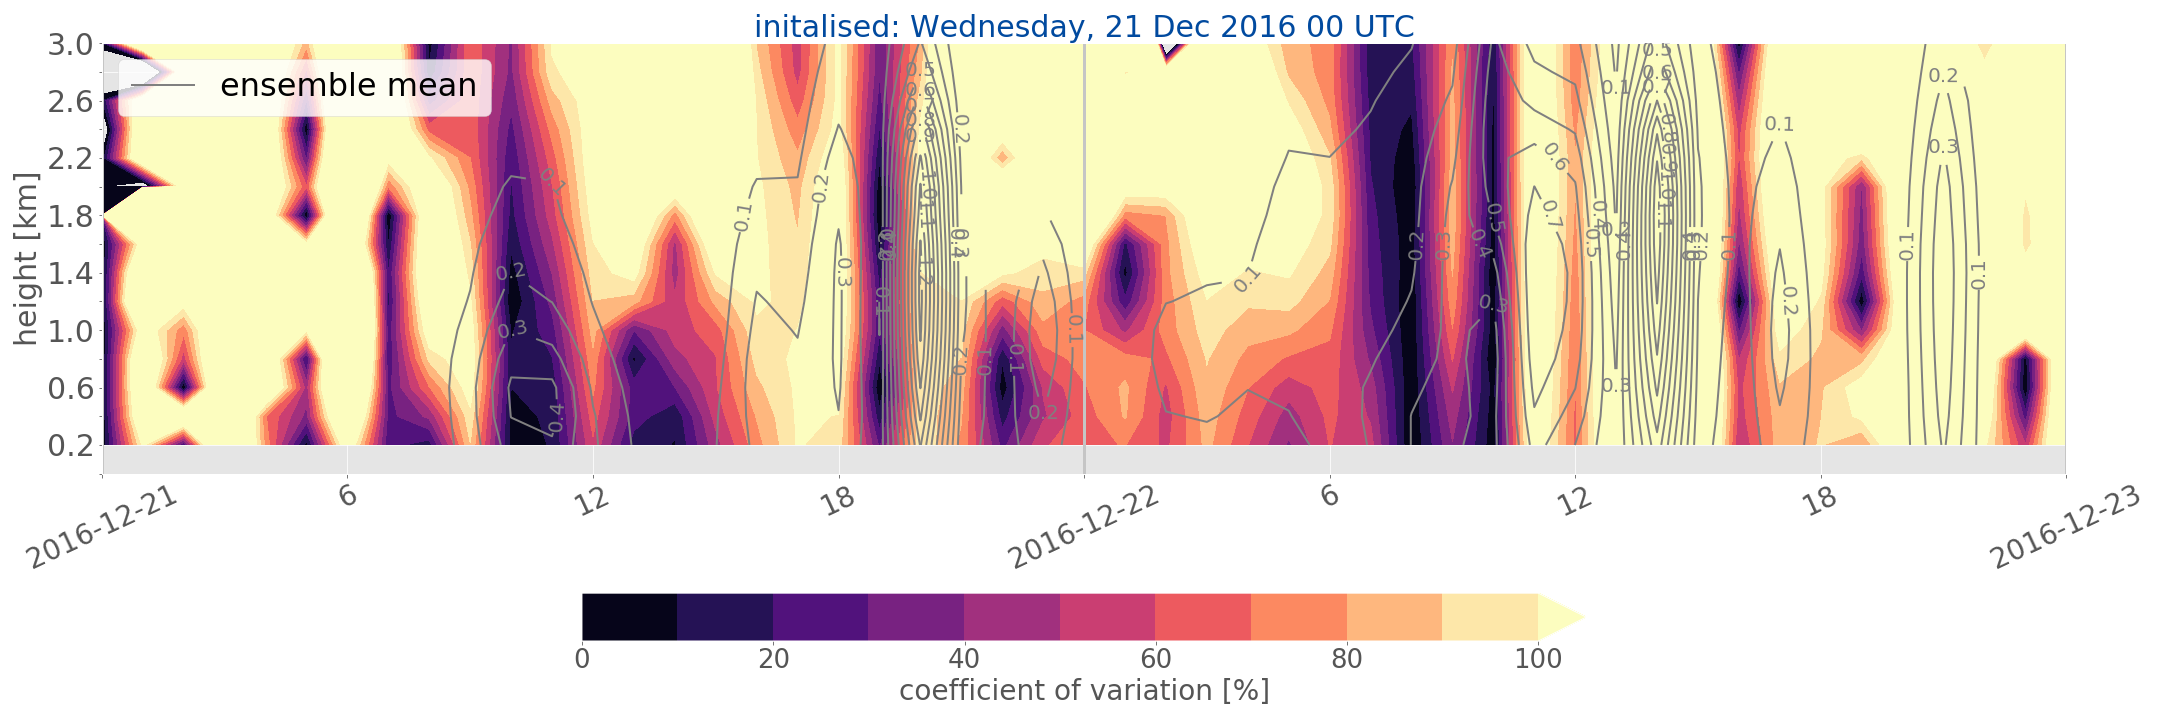
\includegraphics[trim={0.cm 5.3cm 0cm 0cm},clip,width=\textwidth]{./fig_variation/20161221}
			\caption{}\label{fig:ens_vari21}
		\end{subfigure}
       
       % colourbar
     	\begin{subfigure}[t]{\textwidth}		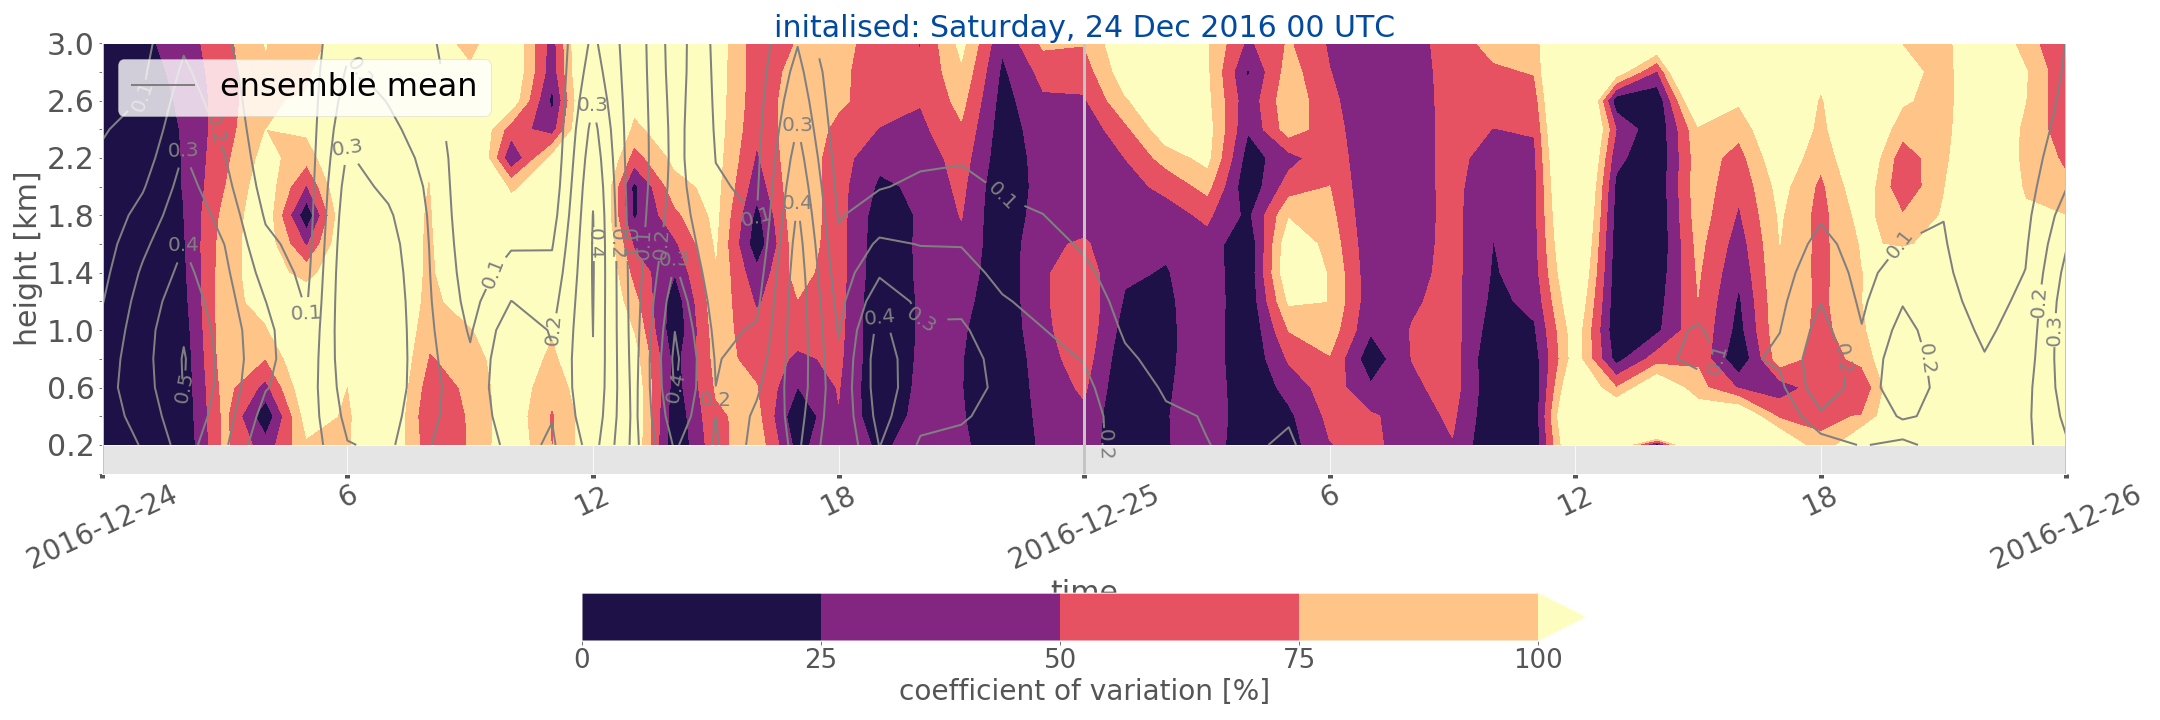
\includegraphics[trim={15.cm 0cm 15cm 21cm},clip,width=\textwidth]{./fig_variation/20161224}
		\end{subfigure}
\end{figure}
\begin{figure}[t]\ContinuedFloat
    % 22/12
		\begin{subfigure}[t]{\textwidth}		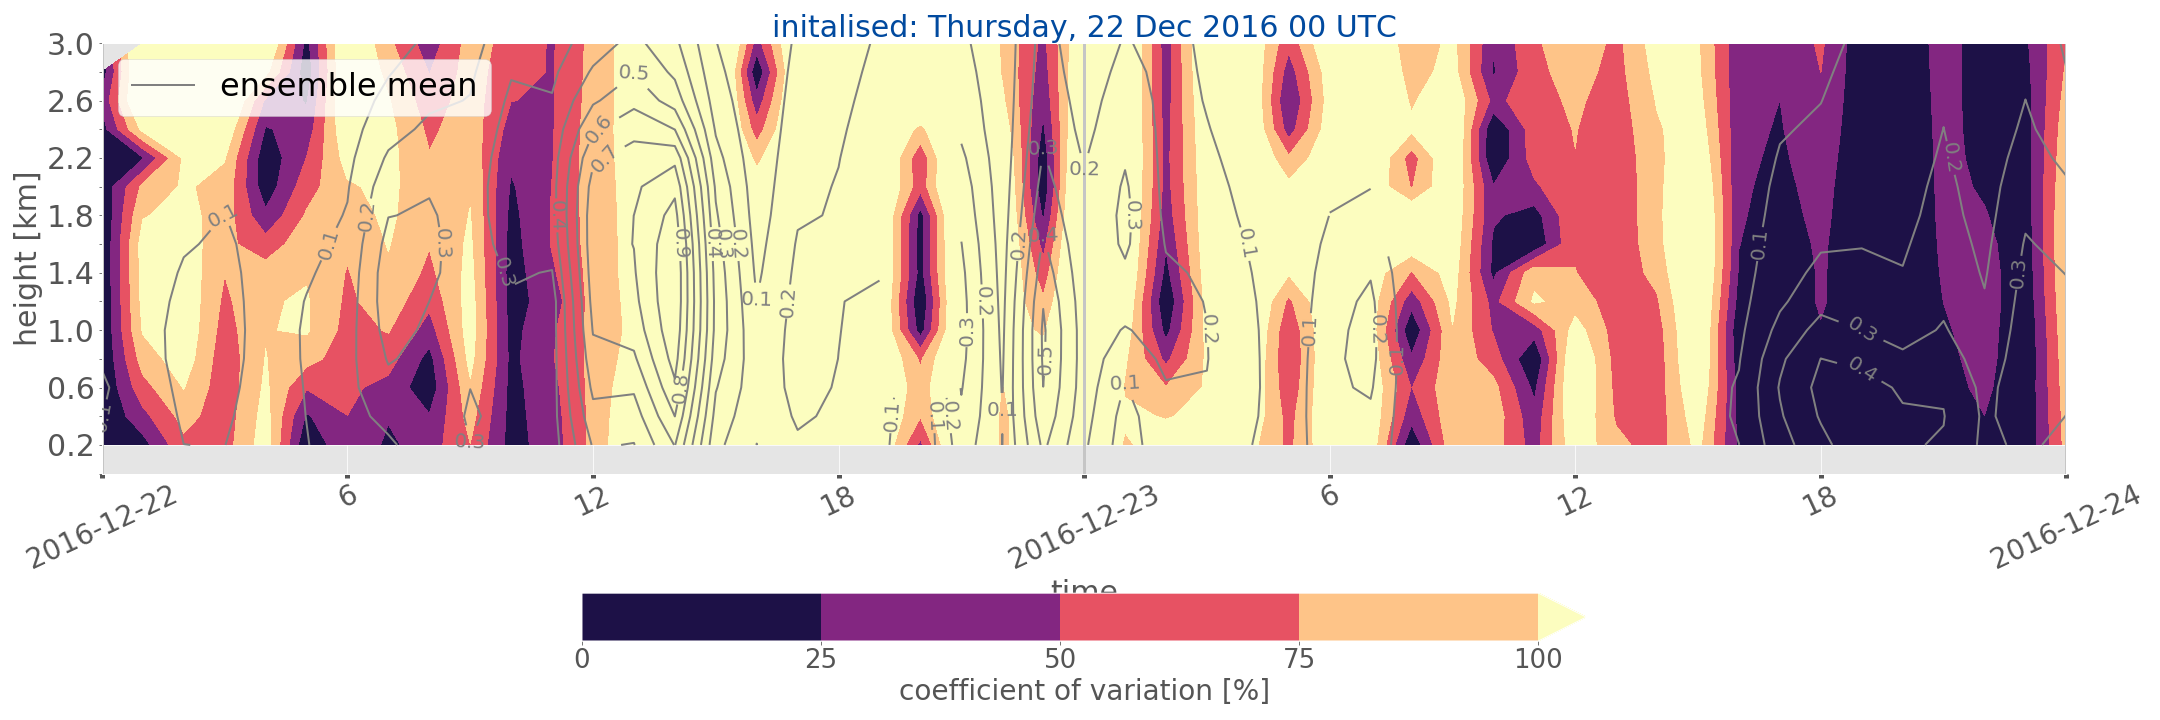
\includegraphics[trim={0.cm 5.3cm 0cm 0cm},clip,width=\textwidth]{./fig_variation/20161222}
			\caption{}\label{fig:ens_vari22}
		\end{subfigure}
    % 23/12
% 		\begin{subfigure}[t]{\textwidth}		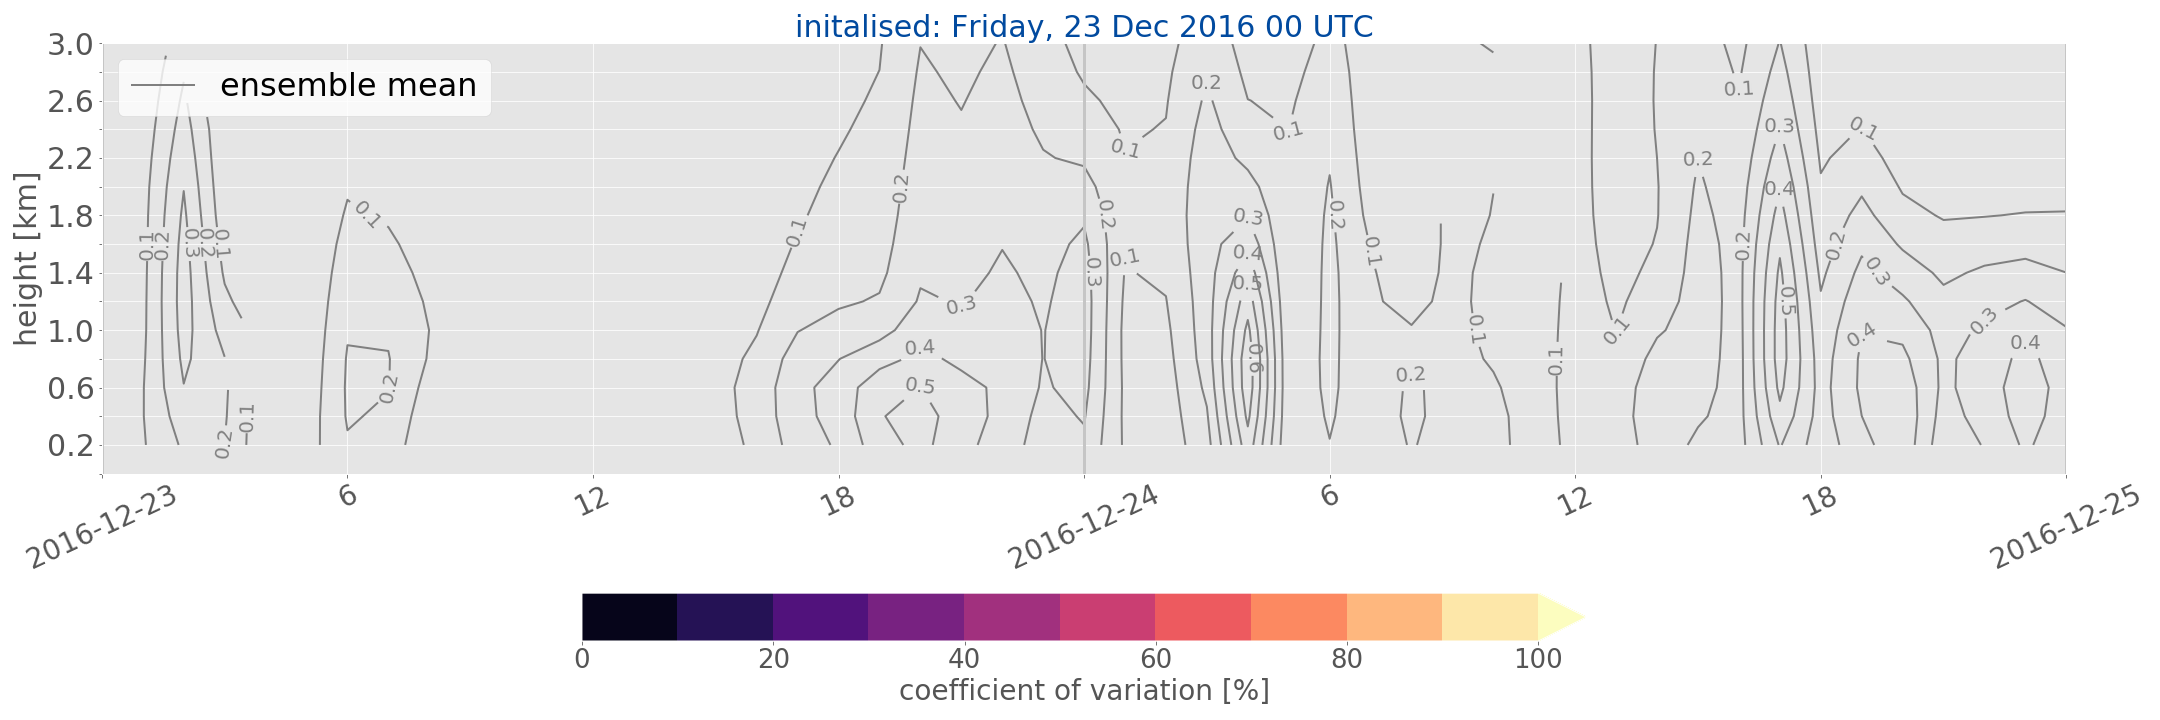
\includegraphics[trim={0.cm 0cm 0cm 0cm},clip,width=\textwidth]{./fig_variation/20161223}
% 			\caption{}\label{fig:ens_vari23}
% 		\end{subfigure}
    % 24/12
		\begin{subfigure}[t]{\textwidth}		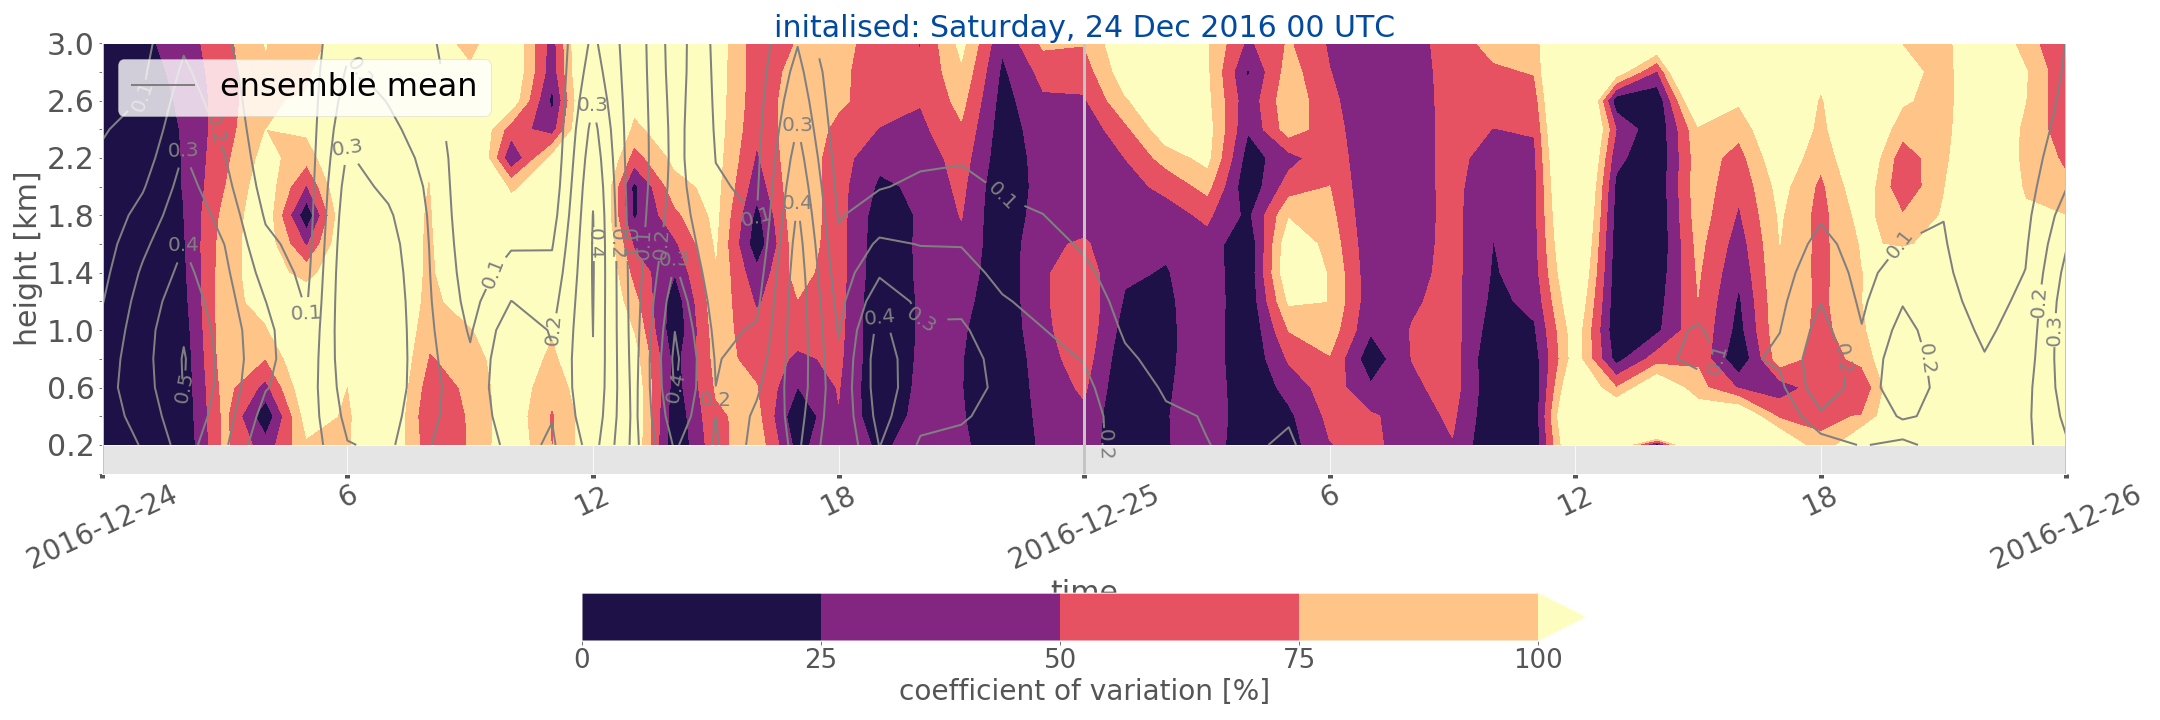
\includegraphics[trim={0.cm 5.3cm 0cm 0cm},clip,width=\textwidth]{./fig_variation/20161224}
			\caption{}\label{fig:ens_vari24}
		\end{subfigure}
        
     % colourbar
     	\begin{subfigure}[t]{\textwidth}		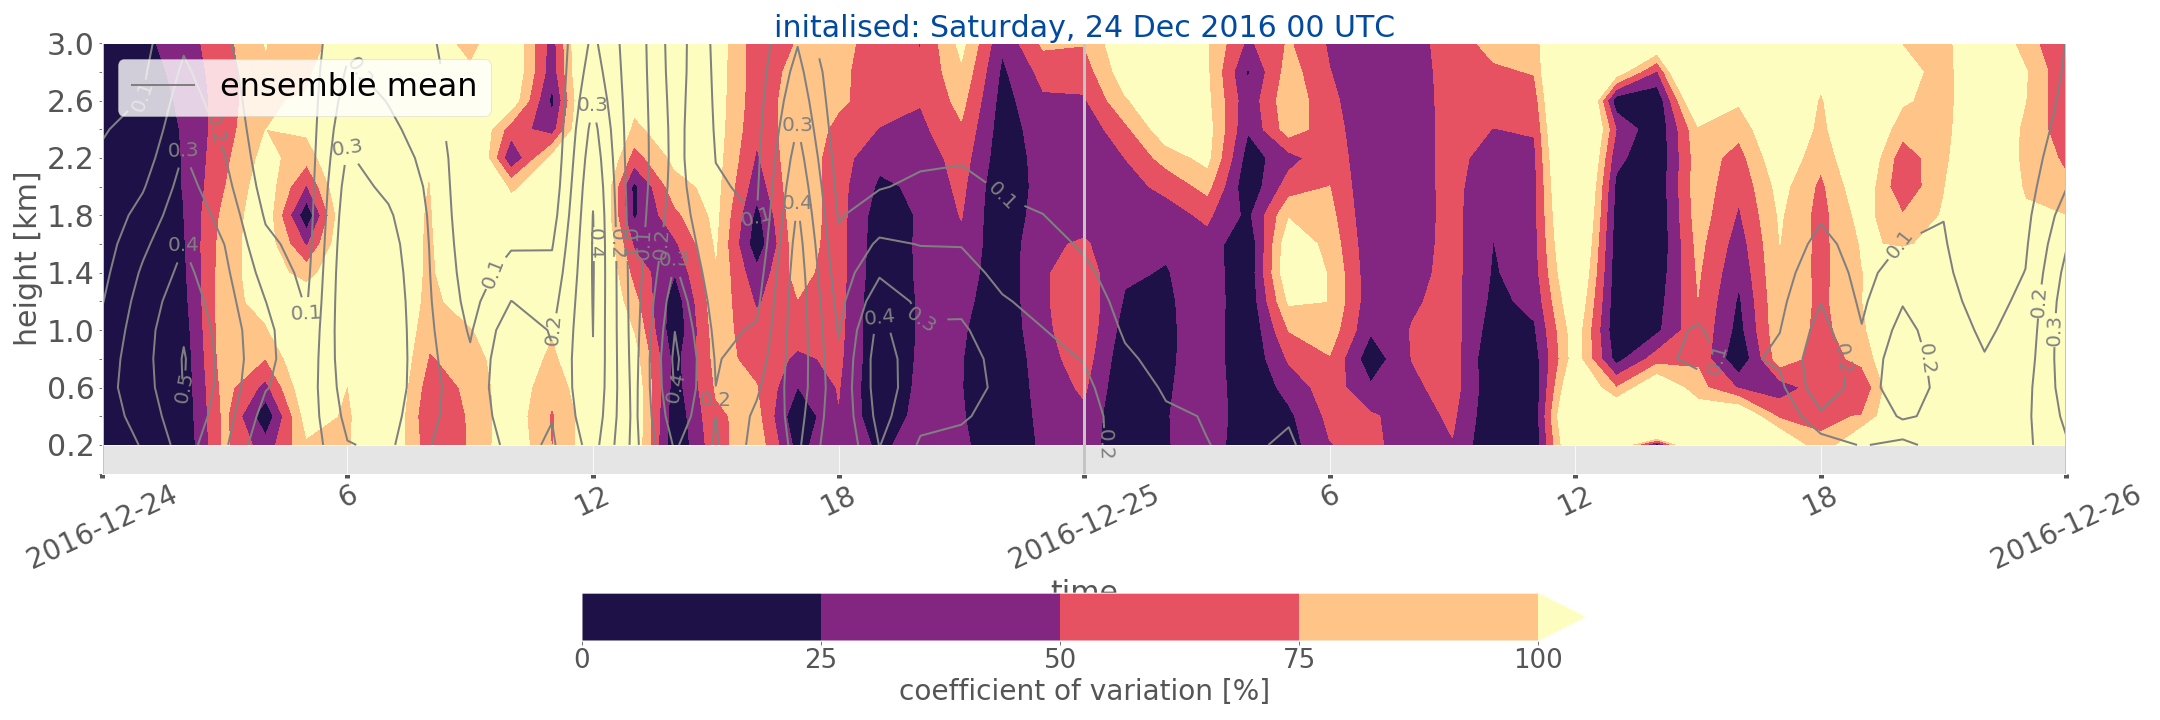
\includegraphics[trim={15.cm 0cm 15cm 21cm},clip,width=\textwidth]{./fig_variation/20161224}
		\end{subfigure}
\end{figure}
\begin{figure}[t]\ContinuedFloat
	\centering
    % 25/12
		\begin{subfigure}[t]{\textwidth}		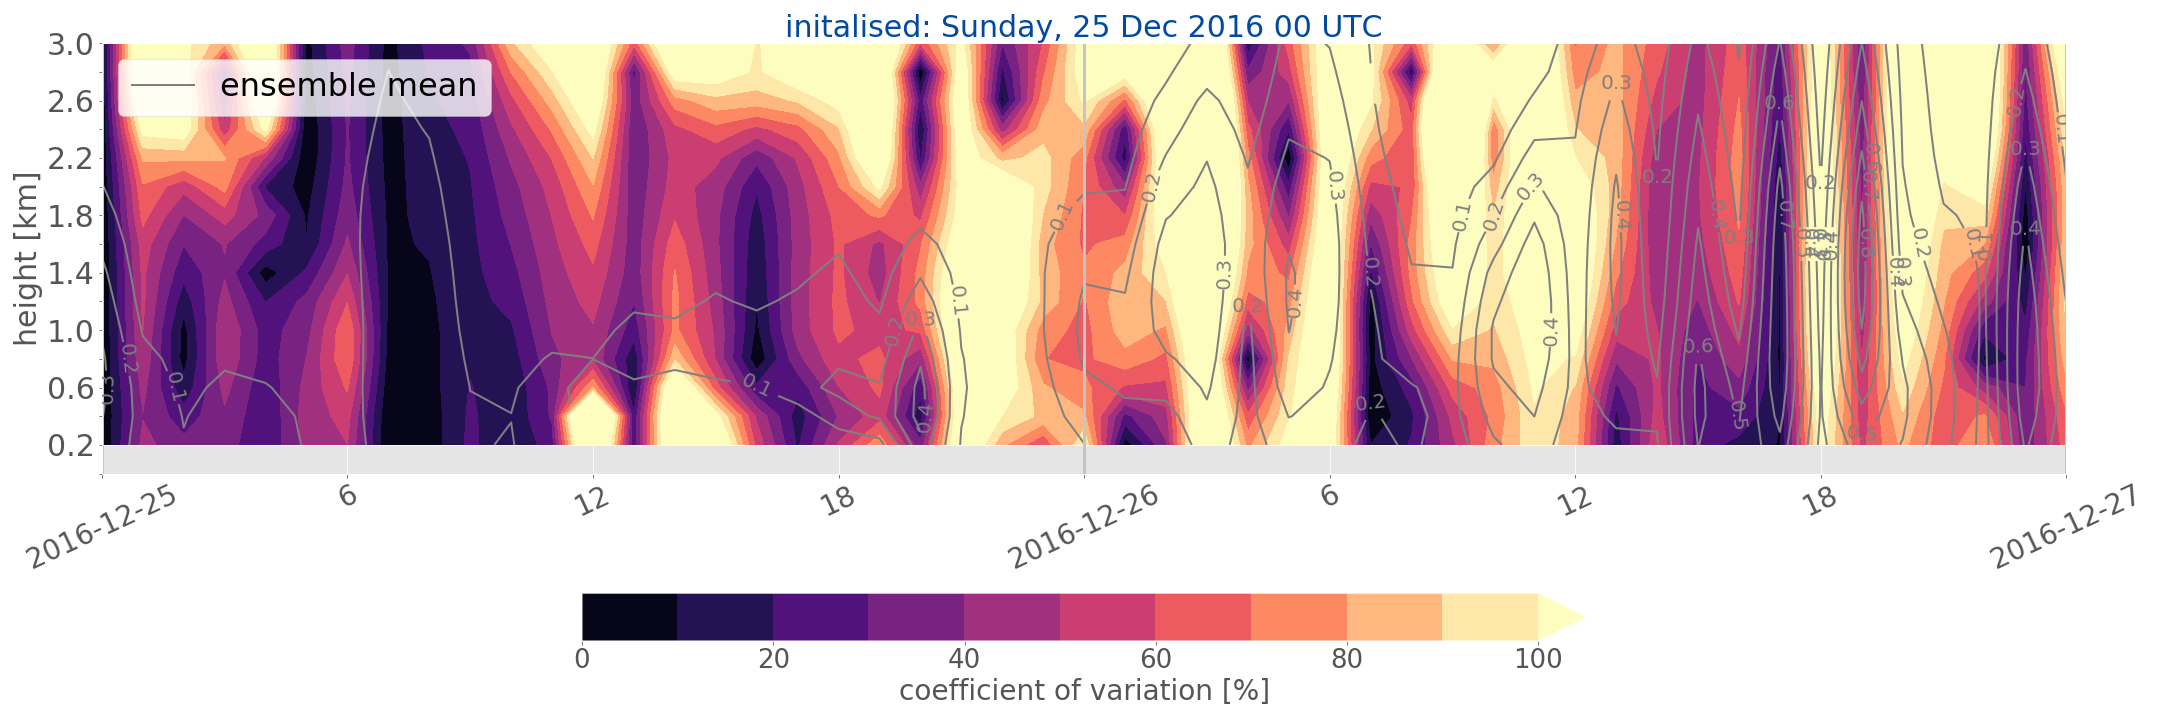
\includegraphics[trim={0.cm 5.3cm 0cm 0cm},clip,width=\textwidth]{./fig_variation/20161225}
			\caption{}\label{fig:ens_vari25}
		\end{subfigure}
    % 26/12
		\begin{subfigure}[t]{\textwidth}		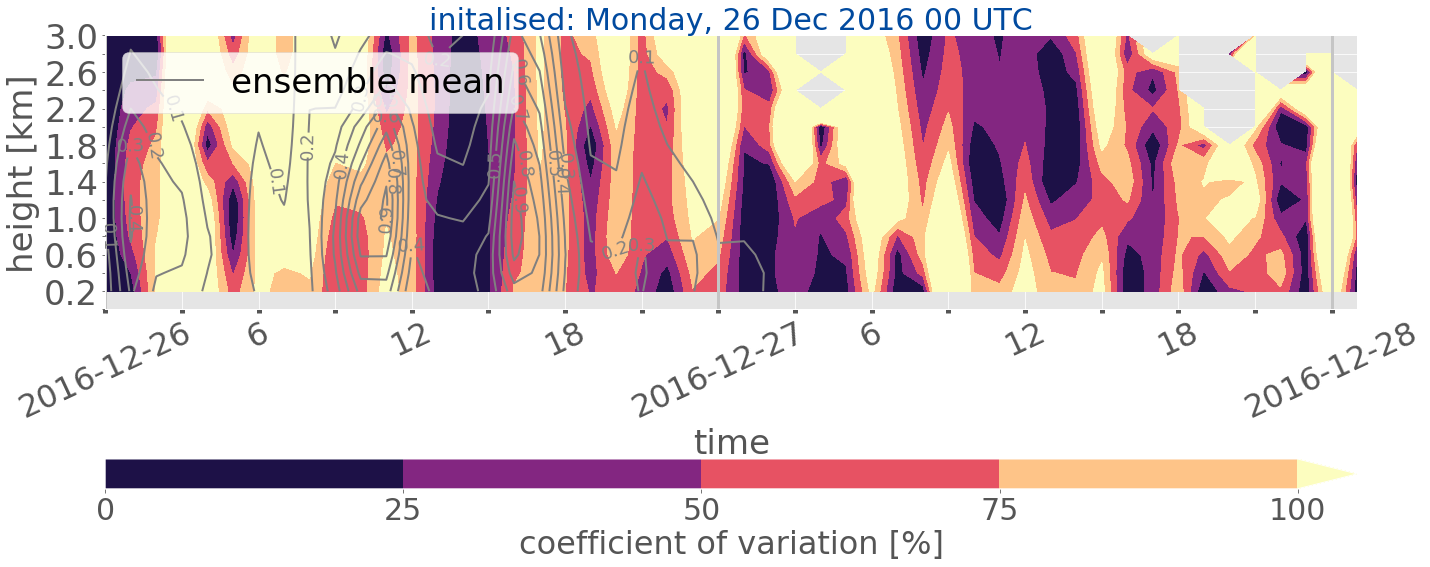
\includegraphics[trim={0.cm 5.3cm 0cm 0cm},clip,width=\textwidth]{./fig_variation/20161226}
			\caption{}\label{fig:ens_vari26}
		\end{subfigure}
%     % 27/12
% 		\begin{subfigure}[t]{\textwidth}		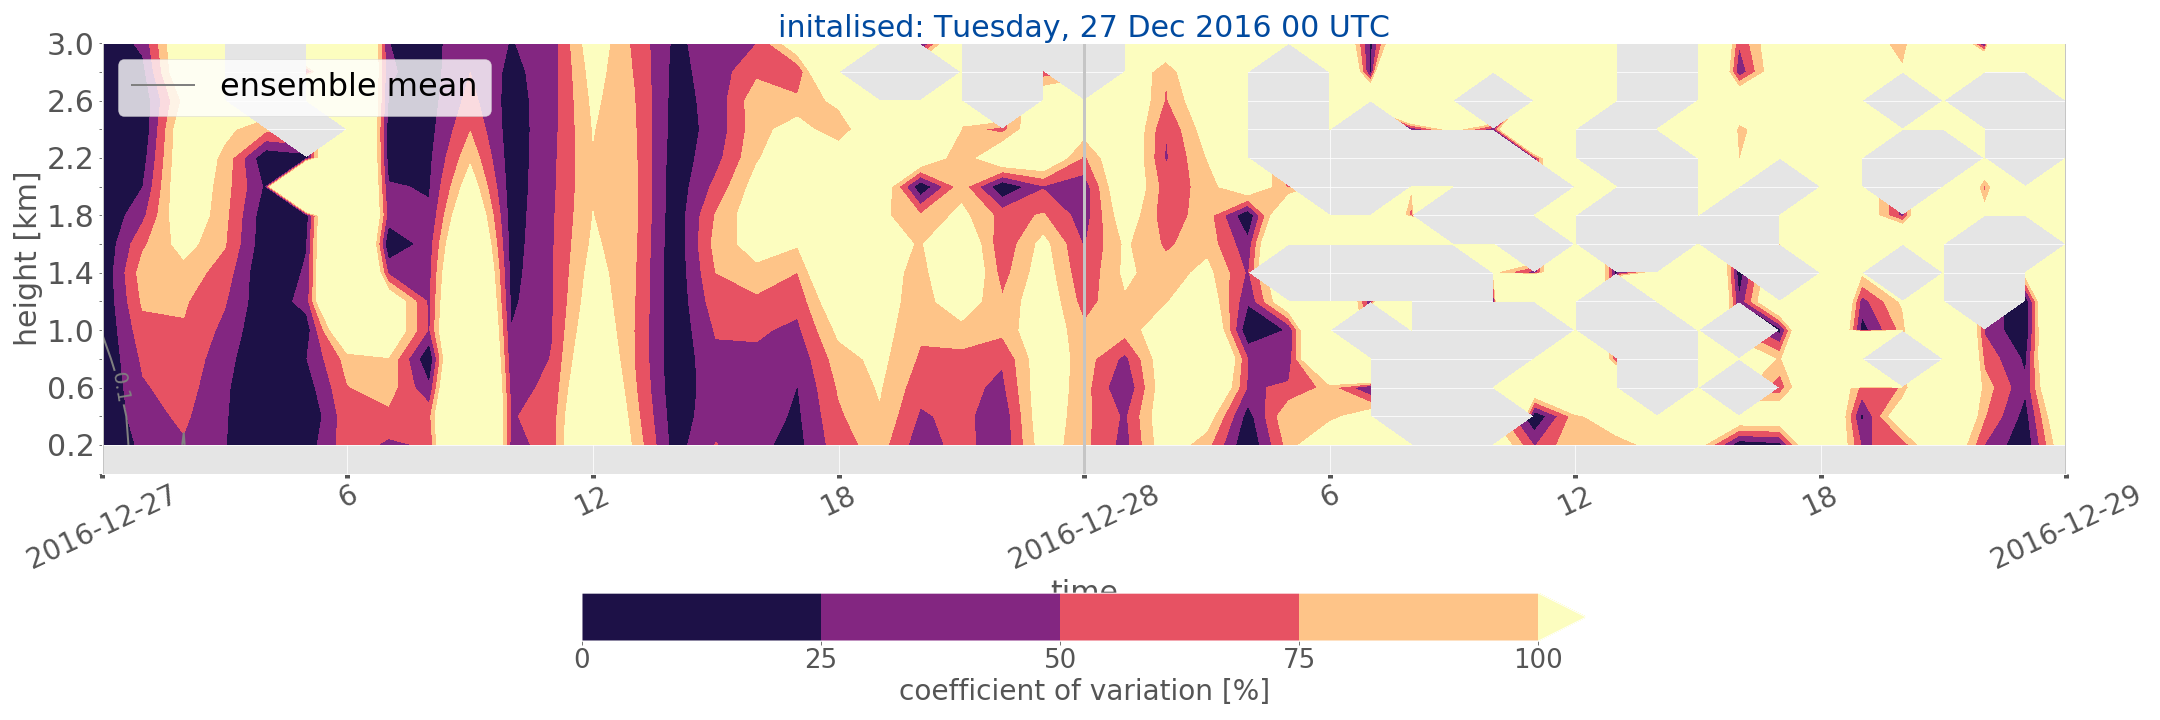
\includegraphics[trim={0.cm 5.3cm 0cm 0cm},clip,width=\textwidth]{./fig_variation/20161227}
% 			\caption{}\label{fig:ens_spread27}
% 		\end{subfigure}
        
    % colourbar
     	\begin{subfigure}[t]{\textwidth}		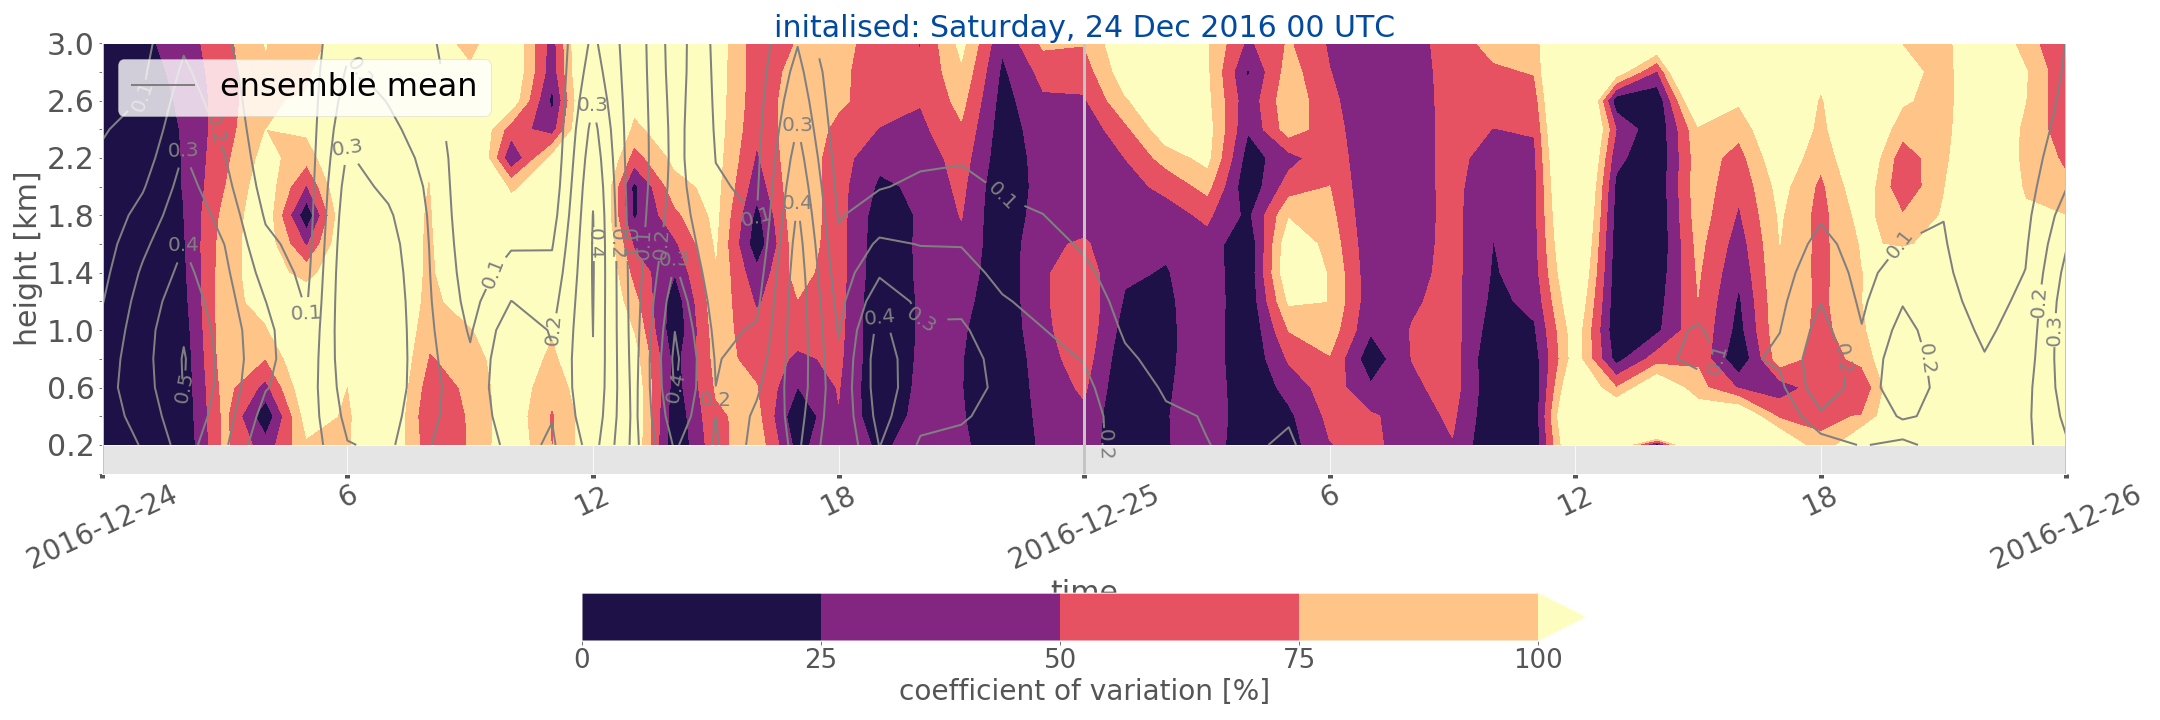
\includegraphics[trim={15.cm 0cm 15cm 21cm},clip,width=\textwidth]{./fig_variation/20161224}
		\end{subfigure}
        \caption{SWC variation of the ten ensemble members of MEPS. The lighter the colour according to the colourbar the higher the variation between the perturbed ensemble members. In grey the ensemble mean of all ten members.}\label{fig:ens_vari}
\end{figure}


%%%%%%%%%%%%%%%%%%%%%%%%%%%%%%%%%%%%%%%%%%%%%%%%%%%%%%%%%%%%%%%%%%%%%%%%%%
To verify how well the ensemble forecast system MEPS has performed, a verification is performed as described in \Cref{sec:ens_mean_spread}. \Cref{fig:ens_vari20,fig:ens_vari21,fig:ens_vari22,fig:ens_vari24,fig:ens_vari25,fig:ens_vari26} show the standard deviation of the ten ensemble members divided by the mean of all ensemble members. 
The grey line in \Cref{fig:ens_vari} shows the ensemble mean as a contour. The darker the colour in \Cref{fig:ens_vari} the more agree the ten ensemble members with the mean. The \SI{23}{\dec} does not exist, because it had too few ensemble members (only six) to create a reasonable verification and therefore is the ensemble mean in \Cref{fig:SWC23} classified as very uncertain. 
\\
In general shows the variation to agree well with the prediction of the up-slope events and be more uncertain about the pulsing part, when west wind is observed. 
\\
The \SI{21}{\dec} contained an up-slope event between \SIrange{9}{13}{\UTC} and a wind change to west followed a pulsing event. The coefficient of variation of the SWC in \Cref{fig:ens_vari20} shows a variation of up to \SI{80}{\percent}, when initialised at \SI{20}{\UTC}. An initialisation on \SI{21}{\dec} gives a better result, were the variation is less than \SI{40}{\percent} for the up-slope part around noon. The variation shows another good agreement around \SI{19}{\UTC}, one hour prior the highest MEPS predicted SWC. 
\\
While the ensemble mean predicted a high SWC at \SIlist{11;14}{\UTC} on the \SI{22}{\dec}, shows the variation of SWC a larger spread around the mean, when the prognosis was initialised on \SI{21}{\dec} (\Cref{fig:ens_vari21}). This follows a high uncertainty of the SWC peak value in \Cref{fig:SWC21}, whereas it is very certain some hours before. The same can be seen in the variation initialised on \SI{22}{\dec}, where it is again no agreement between the different ensemble members for the peaked values. One reason could be the dominance of some ensemble members with high SWC values (compare \Cref{fig:EM09_21} and \ref{fig:EM09_22}). 
\\
All ensemble members agree well with the occurrence of the up-slope storm on \SI{23}{\dec}. The verification in \Cref{fig:ens_vari22} shows little discrepancy below \SI{30}{\percent} and agrees well with the ensemble mean. This is probably due to the fact, that all ten ensemble members forecast the up-slope to occur after \SI{17}{\UTC}, compare \Cref{fig:EM09_22}. While comparing only six ensemble members in \Cref{fig:EM09_23}, one could assume that the uncertainty of all ensemble members during the up-slope storm is low, since all existing ensemble members would agree on the happening of the up-slope storm. No further discussion can be made on this basis, since the presence of fewer ensemble members might lead to incorrect results.
\\
The \SI{24}{\dec} was one of the days, where pulsing of the storm was observed and predicted throughout the day. The variation coefficient of all ten ensemble members in \Cref{fig:ens_vari24} show a good agreement after \SI{14}{\UTC}. The maximum SWC was prognosed at \SI{2}{\UTC} which is still in an area of few variation of the ensemble members around the mean. After that until \SI{14}{\UTC} all ensemble members  disagree. Later, the agreement between the ensemble members increases again, were the overlaid ensemble mean does not fit to the pulsed coefficient of variation. 
\\
In general was the \SI{25}{\dec} a very weak snow storm. \Cref{fig:SWC24} and \Cref{fig:SWC25} gave a very low value of predicted SWC. As \Cref{fig:ens_vari24} is the variability of the ten ensemble members around the mean good until noon, this is when the liquid precipitation appeared. According to \Cref{fig:LWC24} and \ref{fig:LWC25} was the depth of the liquid layer up to \SI{0.8}{\km}. The variation coefficient has a large disagreement below \SI{0.8}{\km}, but above a good agreement of the SWC within all ensemble members is expected. Unfortunately the optimal estimation retrieval is only constructed to retrieve snow. At this point it would be interesting to see, if the MEPS forecast actually covered the real snow content. The verification, initialised on \SI{25}{\dec} shows a well agreement between the weak peak  at \SI{7}{\UTC}. Again, the time when liquid precipitation was observed seems at least be predicted correctly in the depth of the layer in \Cref{fig:ens_vari25}, since the values of the mean must be very small and follow a large discrepancy.
\\
Again, the \SI{26}{\dec} is only comparable until \SI{17}{\UTC}. The two peaks before \SI{18}{\UTC} (\Cref{fig:SWC25}) seem to agree well within all ensemble members, since the variation of SWC is below \SI{50}{\percent} in \Cref{fig:ens_vari25}. Initialised on \SI{26}{\dec} follows that all ensemble member agree well with SWC between \SIlist{12;15}{\UTC}. Whereas the variation for the two peaks at \SIlist{11;16}{\UTC} show a larger disagreement. When looking at \Cref{EM09_26} might this discrepancy from the difference between all ensemble members, only a few agree on the peak at \SI{11}{\UTC} and again, the deterministic forecast (EM0) has the highest SWC.
%
\\[12pt]
Another way to verify an ensemble prediction system is to use the ensemble spread of the SWC, which is just the standard deviation of all ten ensemble members, shown in \Cref{fig:ens_spread}. Here, lighter colours of the SWC show more deviation of the SWC around the ensemble mean and darker colours indicate that the ensemble members are close to the mean. Grey contour lines indicate the ensemble mean of the SWC to see any variations.
\\
As the results in \Cref{fig:ens_spread} show is the spread very low for the up-slope cases (\Cref{fig:ens_spread20,fig:ens_spread21,fig:ens_spread22,fig:ens_spread23}). This means that all ensemble members perform well when the wind is from the east. 
\\
The ensemble spread shows more uncertainty for the pulsing events. 
Initialisation on \SIlist{21;22;26}{\UTC} shows more spread between the different ensemble members (lighter colour in \Cref{fig:ens_spread21}, \ref{fig:ens_spread22}, and \ref{fig:ens_spread26}), especially for the ensemble mean maximum values. On these days the maximum SWC was quite high and reached the overall ensemble mean maximum of \SI{1.24}{\SWC} on \SI{21}{\dec}.
Fewer spread between the ensemble members is shown for the initialisation \SIlist{23;24;25}{\UTC} (\Cref{fig:ens_spread23,fig:ens_spread24,fig:ens_spread25}), when the ensemble mean never reached more than \SI{0.54}{\SWC}.